\begin{figure}[H]
    \centering
    \begin{mdframed}
        \centering
        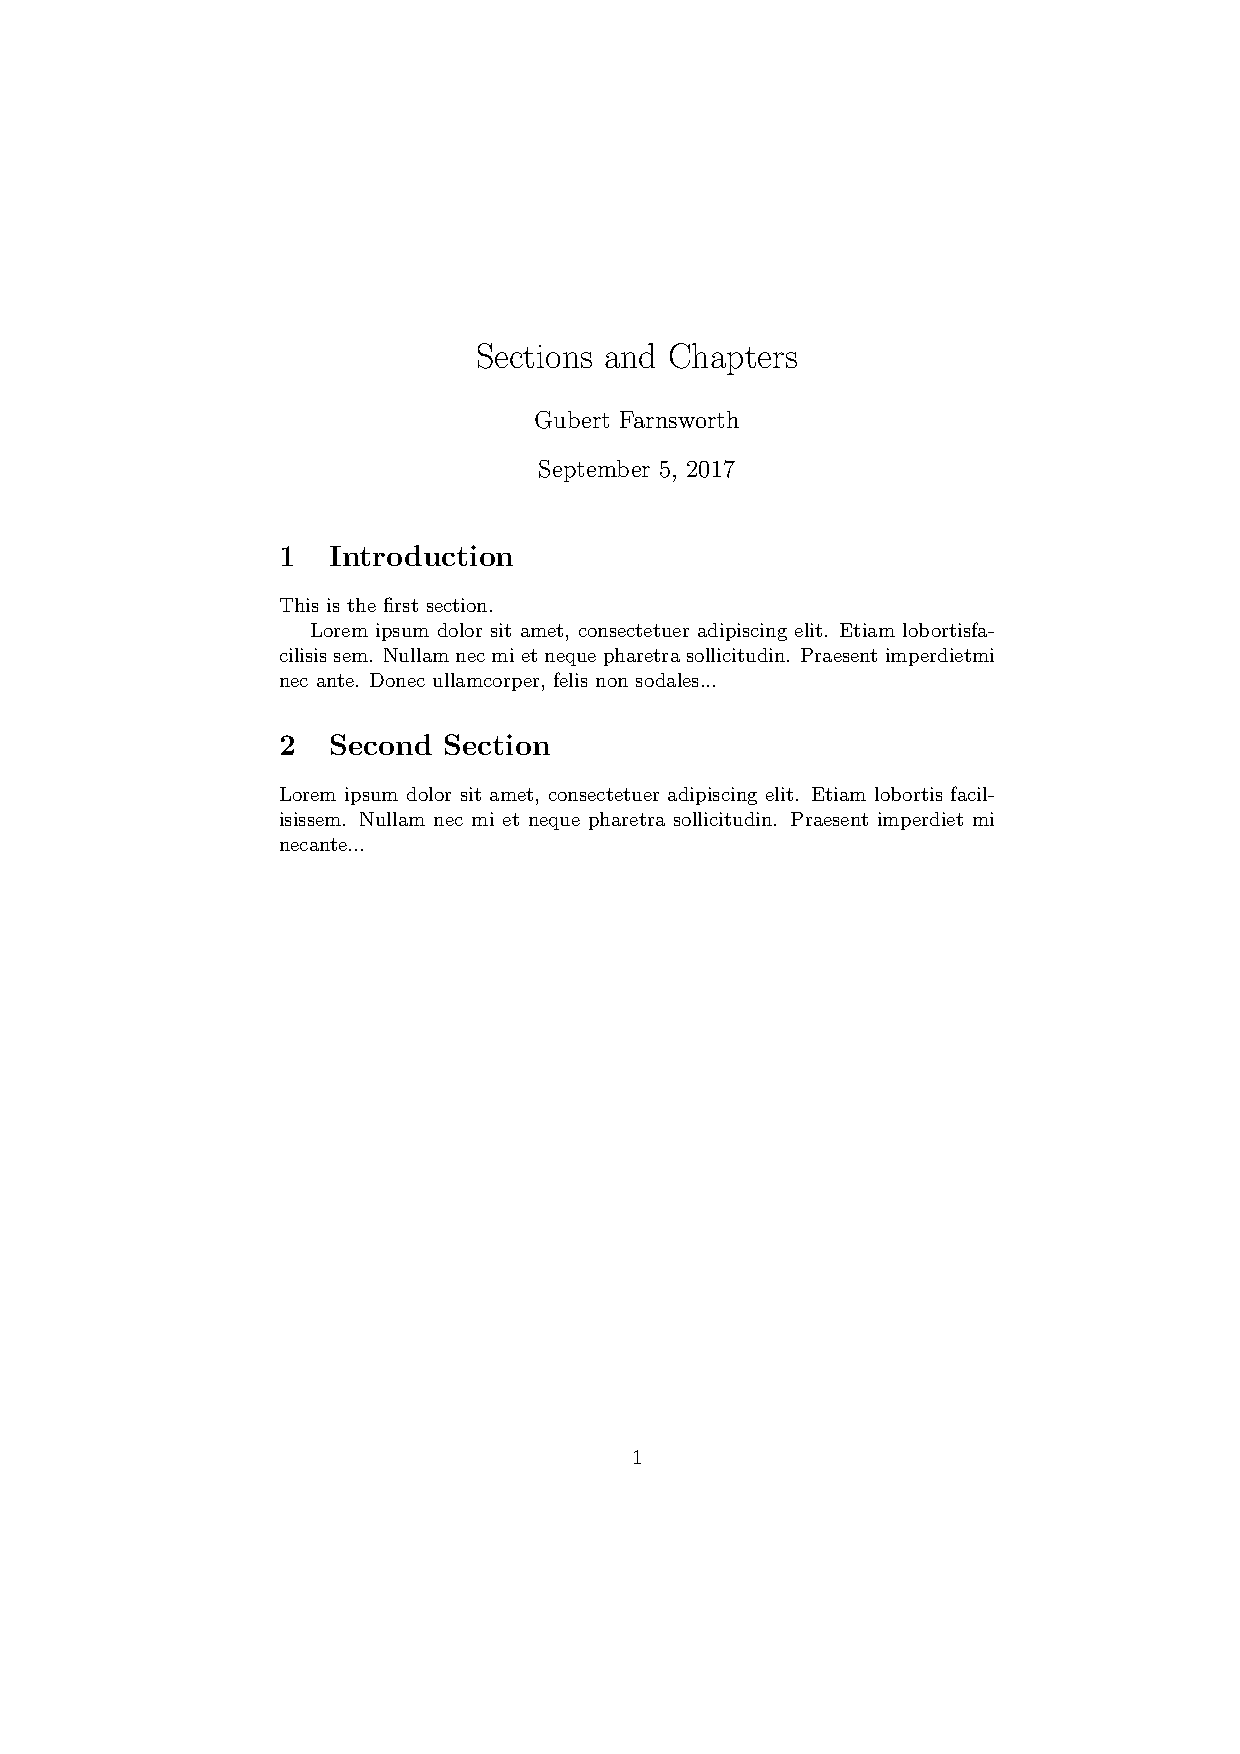
\includegraphics[scale=0.35]{./resources/figures/netl.png}
    \end{mdframed}
    \caption[nETL Architecture]{\textbf{Figure \ref{nETL}: nETL Architecture.} \textit{nETL} is an ETL framework designed to host user-created \textit{Modules} to define \textit{extraction}, \textit{transformation} and \textit{loading} processes. \textit{Modules}, shown in the colored boxes, consist of two parts: a configuration object (a JSON object) and a function that adheres to the specified contract. On startup the \textit{nETL} framework loads modules via the operations via a function made available by the main class. The modules are then cached in main memory by the \textit{nETL} process. A user can then interact with the TaskManager class to create a new task via loading a JSON configuration that makes use of a particular \textit{Module}. Tasks consist of an \textit{Extraction module} configuration, several \textit{Transformation module} configurations and a \textit{Load} configuration. Because modules are created and defined by users, as well as the order in which modules are executed, input/output contracts are also defined by the user, and as such \textit{ETL} processes are infinitely configurable.}
    \label{nETL}
\end{figure}